\chapter{Writing USB Drivers}

This chapter provides documentation and general guidelines for usage of the
refactored USB device driver interface. As such, it is meant for developers of
HelenOS device drivers, who can use it as a reference guide. By intention, this
section abstracts the reader from all modifications to the stack, and focuses
only on the latest state of the interface. All changes to the interface are
described in detail in Chapter \ref{usb-refactoring}.

The reader should note that there exists a similar section in the initial USB
stack documentation. The text in this chapter could be considered an updated
version or extension of that text.


\section{Basics}

This section gives details on the basic structure of USB device drivers, their
role in the system and components they usually interact with.


\subsection{Framework}

USB device drivers use the generic \textit{Device Driver Framework} available in
HelenOS. Because all USB drivers have similar initialization routines, a thin
layer -- specific to USB devices -- was added above the generic one. This layer
mainly serves as a middleware for easy communication with USB host controller
drivers, performing USB specific resource management and enabling device drivers
to initialize endpoint pipes and interact with USB devices. For those reasons,
USB device drivers are recommended to link with \lib{libdrv} and
\lib{libusbdev}, which contain both aforementioned layers respectively.

It is expected that USB device drivers specify in advance not only their
relevant match identifiers, which are used by the Device Manager to pair new
devices with available drivers, but also all endpoints, which shall be present
on the device through a USB driver structure. Later when a new device is found,
a specialized device structure is prepared and pipe abstractions are
initialized.

Device drivers live the same life cycle as any other drivers controlled by the
\textit{Device Manager}. A quick summary follows:
~
\begin{enumerate}
	\item The driver is started at the convenience of the Device Manager if and
	when a compatible device is found. At startup, the driver registers with the
	USB framework, which in turn registers also with the Device Driver
	Framework.

	\item During its lifetime, the driver receives IPC callbacks from the USB
	Framework, informing it about relevant device events. On the basis of these
	events, the driver then communicates with the device and exposes various
	interfaces to other tasks in the system. At this point, the controlled
	device usually becomes visible and useful to the user.

	\item When there is no more need for the driver to run (i.e. no devices to
	control), the Device Manager terminates the driver to save resources.
\end{enumerate}

In the Device Driver Framework, drivers are the consumers of \textit{devices}
and providers of \textit{functions}. This paradigm allows them to expose an
unlimited number of nodes (representing logical or physical units) for every
device they control. The same basic principle holds for USB drivers as well.


\subsection{Device Callbacks}

As explained in the previous section, USB device drivers are informed about
relevant device events by asynchronous IPC callbacks from the USB framework. To
simplify usage, these callbacks are identical to those of the Device Driver
Framework:
~
\begin{description}
	\item[Add Device] This event notifies the driver that a new device has been
	discovered and matched to it. From this point on, the driver is allowed to
	communicate with the device in order to configure it and expose its
	functions to the rest of the system. Further communication with the device
	will likely depend on remote calls originating from other system tasks
	utilizing the exposed interface.

	\item[Remove Device] This event instructs the driver to immediately disallow
	new user operations on a device, terminate all currently running
	operations in a timely manner, and hand device control back to the system,
	as the device will likely be physically removed from the bus in the
	forseeable future.

	\item[Device Gone] This event informs the driver that a device has been
	physically disconnected from the system without a prior \textit{Remove
	Device} event. Since the device is no longer reachable, the driver is to
	force interrupt all user operations, which were running at the time of
	receiving the event and report failure to the callers.
	
	\item[Offline Function] By receiving this event, the driver is asked by the
	system to explicitly transition a specific function exposed by one of its
	controlled devices into the \textit{Offline} state. The meaning of such
	transition might depend on the interpretation of the function. For more
	information, see the Device Driver Framework Documentation.

	\item[Online Function] By receiving this event, the driver is asked by the
	system to explicitly transition a specific function exposed by one of its
	controlled devices into the \textit{Online} state. Again, the meaning of such
	transition might depend on the interpretation of the function. For more
	information, see the Device Driver Framework Documentation.
\end{description}

\begin{figure}
	\centering
	\label{fig:device-states}
	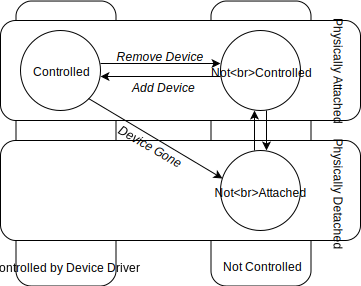
\includegraphics[width=0.5\textwidth]{device-states}
	\caption[Diagram of USB device states and transition events.]{Diagram of USB
	device states and transition events, as perceived by the device driver. Note
	that these states do \textit{not} correspond to USB bus device states (e.g.
	\textit{Configured}, \textit{Addressed}, etc.) in any way.}
\end{figure}

The listed events are delivered to device drivers through function calls to
event handlers specified in the main USB driver operations structure (see
Listing \ref{lst:driver-ops-structure} for a minimal example). The order of
event delivery models the physical lifecycle of the device within the system.
For instance, it is not possible for the \textit{Add Device} event to occur more
than once for the same device in a row. For reference, the exact device states
and transitions between them (corresponding to the events with respective names)
are shown in Figure \ref{fig:device-states}.

Furthermore, since there are no guarantees on the synchronization between calls,
the driver is explicitly responsible for synchronizing accesses to its private
data structures as well as device communication.

\begin{listing}
	\begin{code}
		static int device_add(usb_device_t *dev)
		{
			usb_log_info("Device '%s' added.", usb_device_get_name(dev));
			return EOK;
		}

		static int device_remove(usb_device_t *dev)
		{
			usb_log_info("Device '%s' removed.", usb_device_get_name(dev));
			return EOK;
		}

		static int device_gone(usb_device_t *dev)
		{
			usb_log_info("Device '%s' gone.", usb_device_get_name(dev));
			return EOK;
		}

		static const usb_driver_ops_t driver_ops = {
			.device_add = device_add,
			.device_remove = device_remove,
			.device_gone = device_gone,
		};
	\end{code}
	\caption[Main USB device driver operations structure.]{Main USB device
	driver operations structure with corresponding event handlers. Note that
	events \textit{Offline Function} and \textit{Online Function} do not require
	a handler and can therefore be omitted in the minimal example.}
	\label{lst:driver-ops-structure}
\end{listing}


\section{Device Communication}

In USB, \textit{a pipe} is an abstraction primitive for a communication channel
between a device and a host computer. For the sake of simplicity, the provided
framework relies on a mechanism based on the same abstraction in order to
facilitate communication between device drivers and devices.


\subsection{Endpoint Description}

In order to use pipes, device drivers must first define at least one
\textit{endpoint description}. The purpose of such definition is to specify all
device endpoints, which will be used for communication by the device driver
throughout its lifecycle. For that reason, all descriptions ought to be
specified in advance and referenced in the main device driver structure (for
example of possible endpoint description definition, refer to Listing
\ref{lst:driver-ep-array}).

\begin{listing}
	\begin{code}
		static const usb_endpoint_description_t bulk_in_ep = {
			.transfer_type = USB_TRANSFER_BULK,
			.direction = USB_DIRECTION_IN,
			.interface_class = USB_CLASS_MASS_STORAGE,
			.interface_subclass = USB_MASSSTOR_SUBCLASS_SCSI,
			.interface_protocol = USB_MASSSTOR_PROTOCOL_BBB,
			.flags = 0
		};

		static const usb_endpoint_description_t bulk_out_ep = {
			.transfer_type = USB_TRANSFER_BULK,
			.direction = USB_DIRECTION_OUT,
			.interface_class = USB_CLASS_MASS_STORAGE,
			.interface_subclass = USB_MASSSTOR_SUBCLASS_SCSI,
			.interface_protocol = USB_MASSSTOR_PROTOCOL_BBB,
			.flags = 0
		};

		static const usb_endpoint_description_t *endpoints[] = {
			&bulk_in_ep, &bulk_out_ep, NULL
		};
	\end{code}
	\caption[Main USB device driver endpoint description array]{Main USB device
	driver endpoint description array. This particular example shows two
	\textit{Bulk} endpoints for SCSI mass storage data transfers in both the
	\textit{In} and \textit{Out} directions.}
	\label{lst:driver-ep-array}
\end{listing}

Endpoint description contains information which can be matched to USB endpoint
descriptors in very much the same way as match identifiers are used to pair
devices with device drivers in HelenOS. Following this scheme, the presented USB
framework does most of the heavy lifting for device drivers. When a new device
is added, prior to delivery of the \textit{Add Device} event, all endpoint
descriptions provided by the driver are matched to device endpoints, resulting
in two possible outcomes for every description:
~
\begin{enumerate}
	\item A device endpoint matching the provided description is found and
		\textit{an endpoint mapping} is created.
	\item No device endpoint matches the provided description, hence no mapping is
		created.
\end{enumerate}

Device drivers can later query the result of the matching and if successful,
retrieve the created endpoint mapping, which contains a fully initialized pipe
instance.


\subsection{Pipe I/O}
% TODO


\subsection{Automatic Polling}
% TODO


\section{Utilities}
% TODO

\subsection{Logging}
% TODO

\subsection{Descriptors}
% TODO

\subsection{DMA Buffers}
% TODO


